\documentclass[fleqn,% draft,
a4paper,11pt]{scrbook}

% Document language : english

\newif\ifprinted
\printedfalse

% Police
\usepackage[utf8]{inputenc}

%% Serif font
% \IfFileExists{stix.sty}{%
%   \usepackage[upint]{stix}}%
% {\usepackage{lmodern}
%   \def\coloneq{:=}}

%% Sans font
%\usepackage[scaled=0.875]{helvet}

\usepackage[tt=false]{libertine}
\usepackage[T1]{fontenc}
\usepackage{graphicx}
\usepackage{amsthm}
\usepackage[slantedGreek,cmintegrals,bigdelims,vvarbb,libertine,libaltvw,liby]{newtxmath}
\useosf

\ifprinted
\KOMAoptions{BCOR=0.5cm}
\fi

\recalctypearea


\let\forall\forallAlt
\let\exists\existsAlt
\let\nexists\nexistsAlt

%% Monospace font
%\usepackage[scaled=0.92,varqu,varl]{zi4}
\usepackage[scaled=0.77]{beramono}


% \usepackage{libertine}
% \usepackage[varg,cmintegrals,bigdelims,varbb,libertine]{newtxmath}

\usepackage{ifdraft}

\usepackage{chngcntr}
\usepackage{tocvsec2}

\KOMAoptions{chapterprefix=true}
\KOMAoptions{headsepline=true}
\KOMAoptions{index=toc}
%\KOMAoptions{bibliography=totocnumbered}
%\addtokomafont{chapter}{\centering}
% \ifdraft{\KOMAoptions{twoside=false}}{}
\renewcommand*{\partformat}{\partname~\thepart}
\renewcommand*{\partpagestyle}{empty}
\renewcommand*{\chapterformat}{\chapappifchapterprefix~\thechapter\\\rule{\linewidth}{1.5pt}\\}


%\KOMAoptions{numbers=noenddot}
\renewcommand*{\figureformat}{\figurename~\thefigure}
\renewcommand*{\tableformat}{\tablename~\thetable}
%\renewcommand*{\captionformat}{.}

%\KOMAoptions{parskip=half*}

\newcommand{\chappreamble}[1]{\textit{\noindent #1}\leavevmode\vspace{\baselineskip}}

\newenvironment{chapabstract}{}{}



% \usepackage{titlesec}
% \titleformat{\chapter}[display]

\usepackage[final]{listings}

\usepackage[style=alphabetic,maxnames=4,backend=bibtex,
backref=true% ,noadjust
,
firstinits=true]{biblatex}
%   \makeatletter
%   \def\@citex#1[#2]#3{% 
%     \@safe@activestrue\edef\@tempd{#1}\@safe@activesfalse
%     \@safe@activestrue\edef\@tempe{#3}\@safe@activesfalse
%     \org@@citex{\@tempd}[#2]{\@tempe}}%
%   \makeatother
%\addbibresource{MyBiblio.bib}

%\makeatletter
% \def\url@leostyle{%
%   \@ifundefined{selectfont}{\def\UrlFont{\sf}}{\def\UrlFont{\footnotesize\ttfamily}}}
% \makeatother
%% Now actually use the newly defined style.
% \urlstyle{leo}

\usepackage{relsize}
\appto{\bibsetup}{\emergencystretch=1em}
\renewcommand*{\UrlFont}{\itshape}
\appto{\biburlsetup}{%
  \renewcommand*{\UrlFont}{\smaller[0.5]
    \itshape% \ttfamily
    %\normalfont\itshape
  }}

\makeindex

\usepackage{titling}
\title{Tableaux Comparatifs}
\author{Luc Sapin}
\date{\today}

%Package pour avoir des liens hyper-texte dans les fichiers Pdf 
%A mettre en dernier 
%Pose parfois problème 
% \usepackage[unicode,final% ,ocgcolorlinks
% ]{hyperref}
% \usepackage{footnotebackref}

\usepackage[final]{hyperref}

\hypersetup{%
  pdfinfo={
    Title={\thetitle},
    Author={\theauthor} },
  % frenchlinks,
  linkcolor=purple,
  citecolor=teal,
  %ocgcolorlinks
  %urlcolor={magenta!50!black},
  % menucolor=purple
}
\ifprinted
\hypersetup{colorlinks=false}
\else
\hypersetup{colorlinks}
\fi



% \tikzexternalize[mode=list and make,up to date check=md5, prefix=figures/]
% \pgfkeys{/pgf/images/include external/.code={\includegraphics{#1}}}


\begin{document}
\maketitle
\chapter*{}
\label{cha:cr-reu}
\section*{Vendredi 23 mars 2018}
tableau de comparaison des résultats entre les points de départ/arrivée EMB et L2.\\


\begin{tabular}{|c||c|c||c|c||c|c|}
	\hline
	\textbf{Outbound} & \multicolumn{2}{c||}{$t_{0o}$} &  \multicolumn{2}{c||}{$dt_{1o}$} & \multicolumn{2}{c|}{$dt_{fo}$} \\
	\hline
	Asteroid & EMB & L2 & EMB & L2 & EMB & L2 \\
	\hline
	1 & 5.45e+03 & -19.81 & 1.16e+02 & 1.95e+02 & 3.70e+02 & 1.80e+02 \\
	\hline
	2 & 5.95e+03 & 6.19e+03 & 3.35e+02 & 1.32e+02 & 3.48 & 1.26e+02 \\
	\hline
	3 & 4.04e+03 & 3.63e+03 & 98.17 & 1.24e+02 & 1.10e+02 & 1.41e+02 \\
	\hline
	4 & 2.41e+03 & 3.27e+03 & 2.39e+02 & 90.04 & 1.94e+02 & 89.81 \\
	\hline
	5 & 2.50e+03 & 3.29e+03 & 3.18e+02 & 85.23 & 1.26e+02 & 88.43 \\
	\hline
	6 & 5.87e+03 & 6.16e+03 & 1.09e+02 & 1.12e+02 & 1.04e+02 & 1.44e+02 \\
	\hline
	7 & 6.56e+03 & 6.22e+03 & 1.14e+02 & 86.73 & 1.58e+02 & 1.49e+02 \\
	\hline
	8 & 6.37e+02 & 5.13e+03 & 2.22e+02 & 1.70e+02 & 82.72 & 1.36e+02 \\
	\hline
	9 & 4.40e+03 & 1.83e+03 & 1.41e+02 & 1.57e+02 & 1.40e+02 & 1.38e+02 \\
	\hline
	10 & 2.93e+03 & 2.57e+03 & 1.03e+02 & 1.85e+02 & 99.95 & 60.44 \\
	\hline
\end{tabular}

\bigbreak
\begin{figure}
	\begin{minipage}[c]{.5\linewidth}
		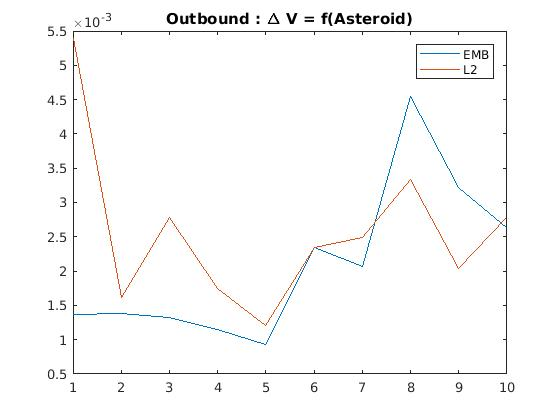
\includegraphics[width=1\textwidth]{OutboundDeltaV10Ast.jpg} \\	
	\end{minipage}\hfill
	\begin{minipage}[c]{.5\linewidth}
		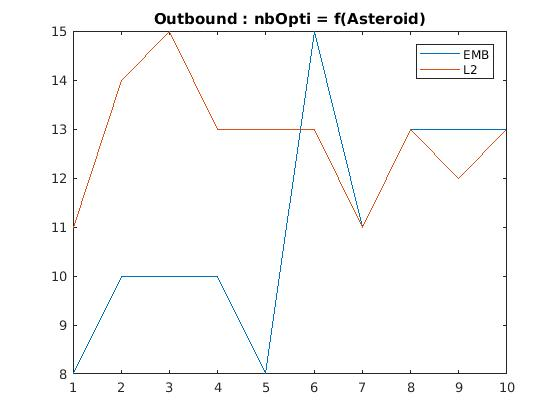
\includegraphics[width=1\textwidth]{OutboundnbOpti10Ast.jpg}	
	\end{minipage}
\end{figure}


\end{document}